\subsection{Debiasing Conceptor}
In this paper, we will compare our work with the debiasing conceptor \cite{karve2019conceptor}. Given a set of gendered words $V:=\{v_1,v_2,\dots,v_n\}$ and their embeddings $E \in R^{n\times d}$, gender bias can be mitigated by multiplying the debiasing conceptor matrix$\neg C= I-C$, where $C$ is the conceptor matrix that minimizes the objective
\begin{eqnarray}
||E-CE||^2_F+\alpha^{-2}||E||^2_F
\end{eqnarray}
where $\alpha^{-2}$ is a scalar parameter. $C$ has an analytical solution
\begin{eqnarray}
C=\frac{1}{n}EE^T(\frac{1}{n}EE^T+\alpha^{-2}I)^{-1}
\end{eqnarray}
Intuitively, C is a soft projection matrix on the linear subspace where the word embeddings have the maximum bias.
\subsection{Hard Debasing}
We will also compare the hard debiasing method proposed by \cite{mu2018all}, which is originally a postprocessing technique for improving word representations. \cite{karve2019conceptor} adopted it as a straightforward debiasing method. Hard debiasing relies upon assuming that the first principal component of the considered vectors is a meaningful gender direction. This simple debiasing method uses PCA to obtain the first principal component from the embeddings of gendered words, and project it off.

\subsection{DensRay}
DensRay is an analytical method for identifying the
embedding subspace of certain linguistic features. We aim to
identify the "gender subspace" using a set of gendered words
$V:=\{v_1,v_2,\dots,v_n\}$ and their embeddings $E \in
R^{n\times d}$, thus for word $v_i$ we have the
corresponding embedding vector $e_{v_i}$. We
introduce a function $l$ for the gender attribute:
$l:V\to \{-1,1\}$;
e.g. $l(father)=1$, $l(sister)=-1$. The objective of DensRay
is to find an orthogonal matrix $Q\in R^{d\times d}$ such
that $EQ$ is gender-interpretable, specifically, the first
$k$ dimensions can be interpreted as the gender subspace.

Let $L_{=}:=\{(v,w)\in V\times V|l(v)=l(w)\}$ and define
$L_{\neq}$ analogously.  The DensRay objective
in \eqref{densray1} is to maximize the distance of the word
pairs from the same gender group ($L_{=}$) and minimize the
distance of the word pairs from the different gender group
($L_{\neq}$).
\begin{eqnarray}
\max\limits_{q} 
\sum_{(v,w)\in L_{\neq}}\alpha_{\neq}||q^Td_{vw}||^2_2
-\sum_{(v,w)\in L_{=}}\alpha_{=}||q^Td_{vw}||^2_2
\eqlabel{densray1}
\end{eqnarray}
where we define $d_{vw}:=e_v-e_w$. We also have $q\in R^d$
and $q^Tq=1$ since $Q$ is orthogonal. $\alpha_{\neq},\alpha_{=}\in [0,1]$ are hyperparameters. Observing that $||x||^2_2=x^Tx$, objective \eqref{densray1} can be simplified to:
\begin{eqnarray}
\max \limits_{q} q^T(
\sum_{(v,w)\in L_{\neq}}\alpha_{\neq}||d_{vw}d_{vw}^T||^2_2-\sum_{(v,w)\in L_{=}}\alpha_{=}||d_{vw}d_{vw}^T||^2_2)q=:\max\limits_{q} q^TAq
\eqlabel{eq:densray2}
\end{eqnarray}

This objective is maximizing the Rayleigh quotient of $A$ and $q$. Since $A$ is symmetric, we can get an analytical solution $q$ by the eigenvector with the max eigenvalue of $A$ \cite{horn1990matrix}. Thus the matrix of $k$ eigenvectors of $A$ ordered by the corresponding eigenvalues yields the matrix $Q$.
\subsection{Removing Gender Information}

All prior methods yield a gender dimension $q \in R^d$. In a contextualized language model like BERT each layer yields a contextualized embedding matrix $X \in R^{t \times d}$ where $t$ is the length of the sentence. To debias representations we simply zero out the projected values on $q$ for each position, that is we set $X^{\text{debiased}}_i = X_i -  (X_i^\intercal q) q$ for each position $i$.

\seclabel{artexample}
 \figref{fig:example} shows artificially created two dimensional embeddings. The lines show the gender directions identified by hard debiasing, debiasing conceptor, and DensRay. 
 
 DensRay separates the gendered words into two gender groups to produce a meaningful gender direction by objective \eqref{eq:densray2}, while debiasing conceptor and hard debiasing compute the subspace with the whole gendered words set. Theoretically, they may fail to identify the correct gender direction in some cases. 
\begin{figure}[h]
	\centering
	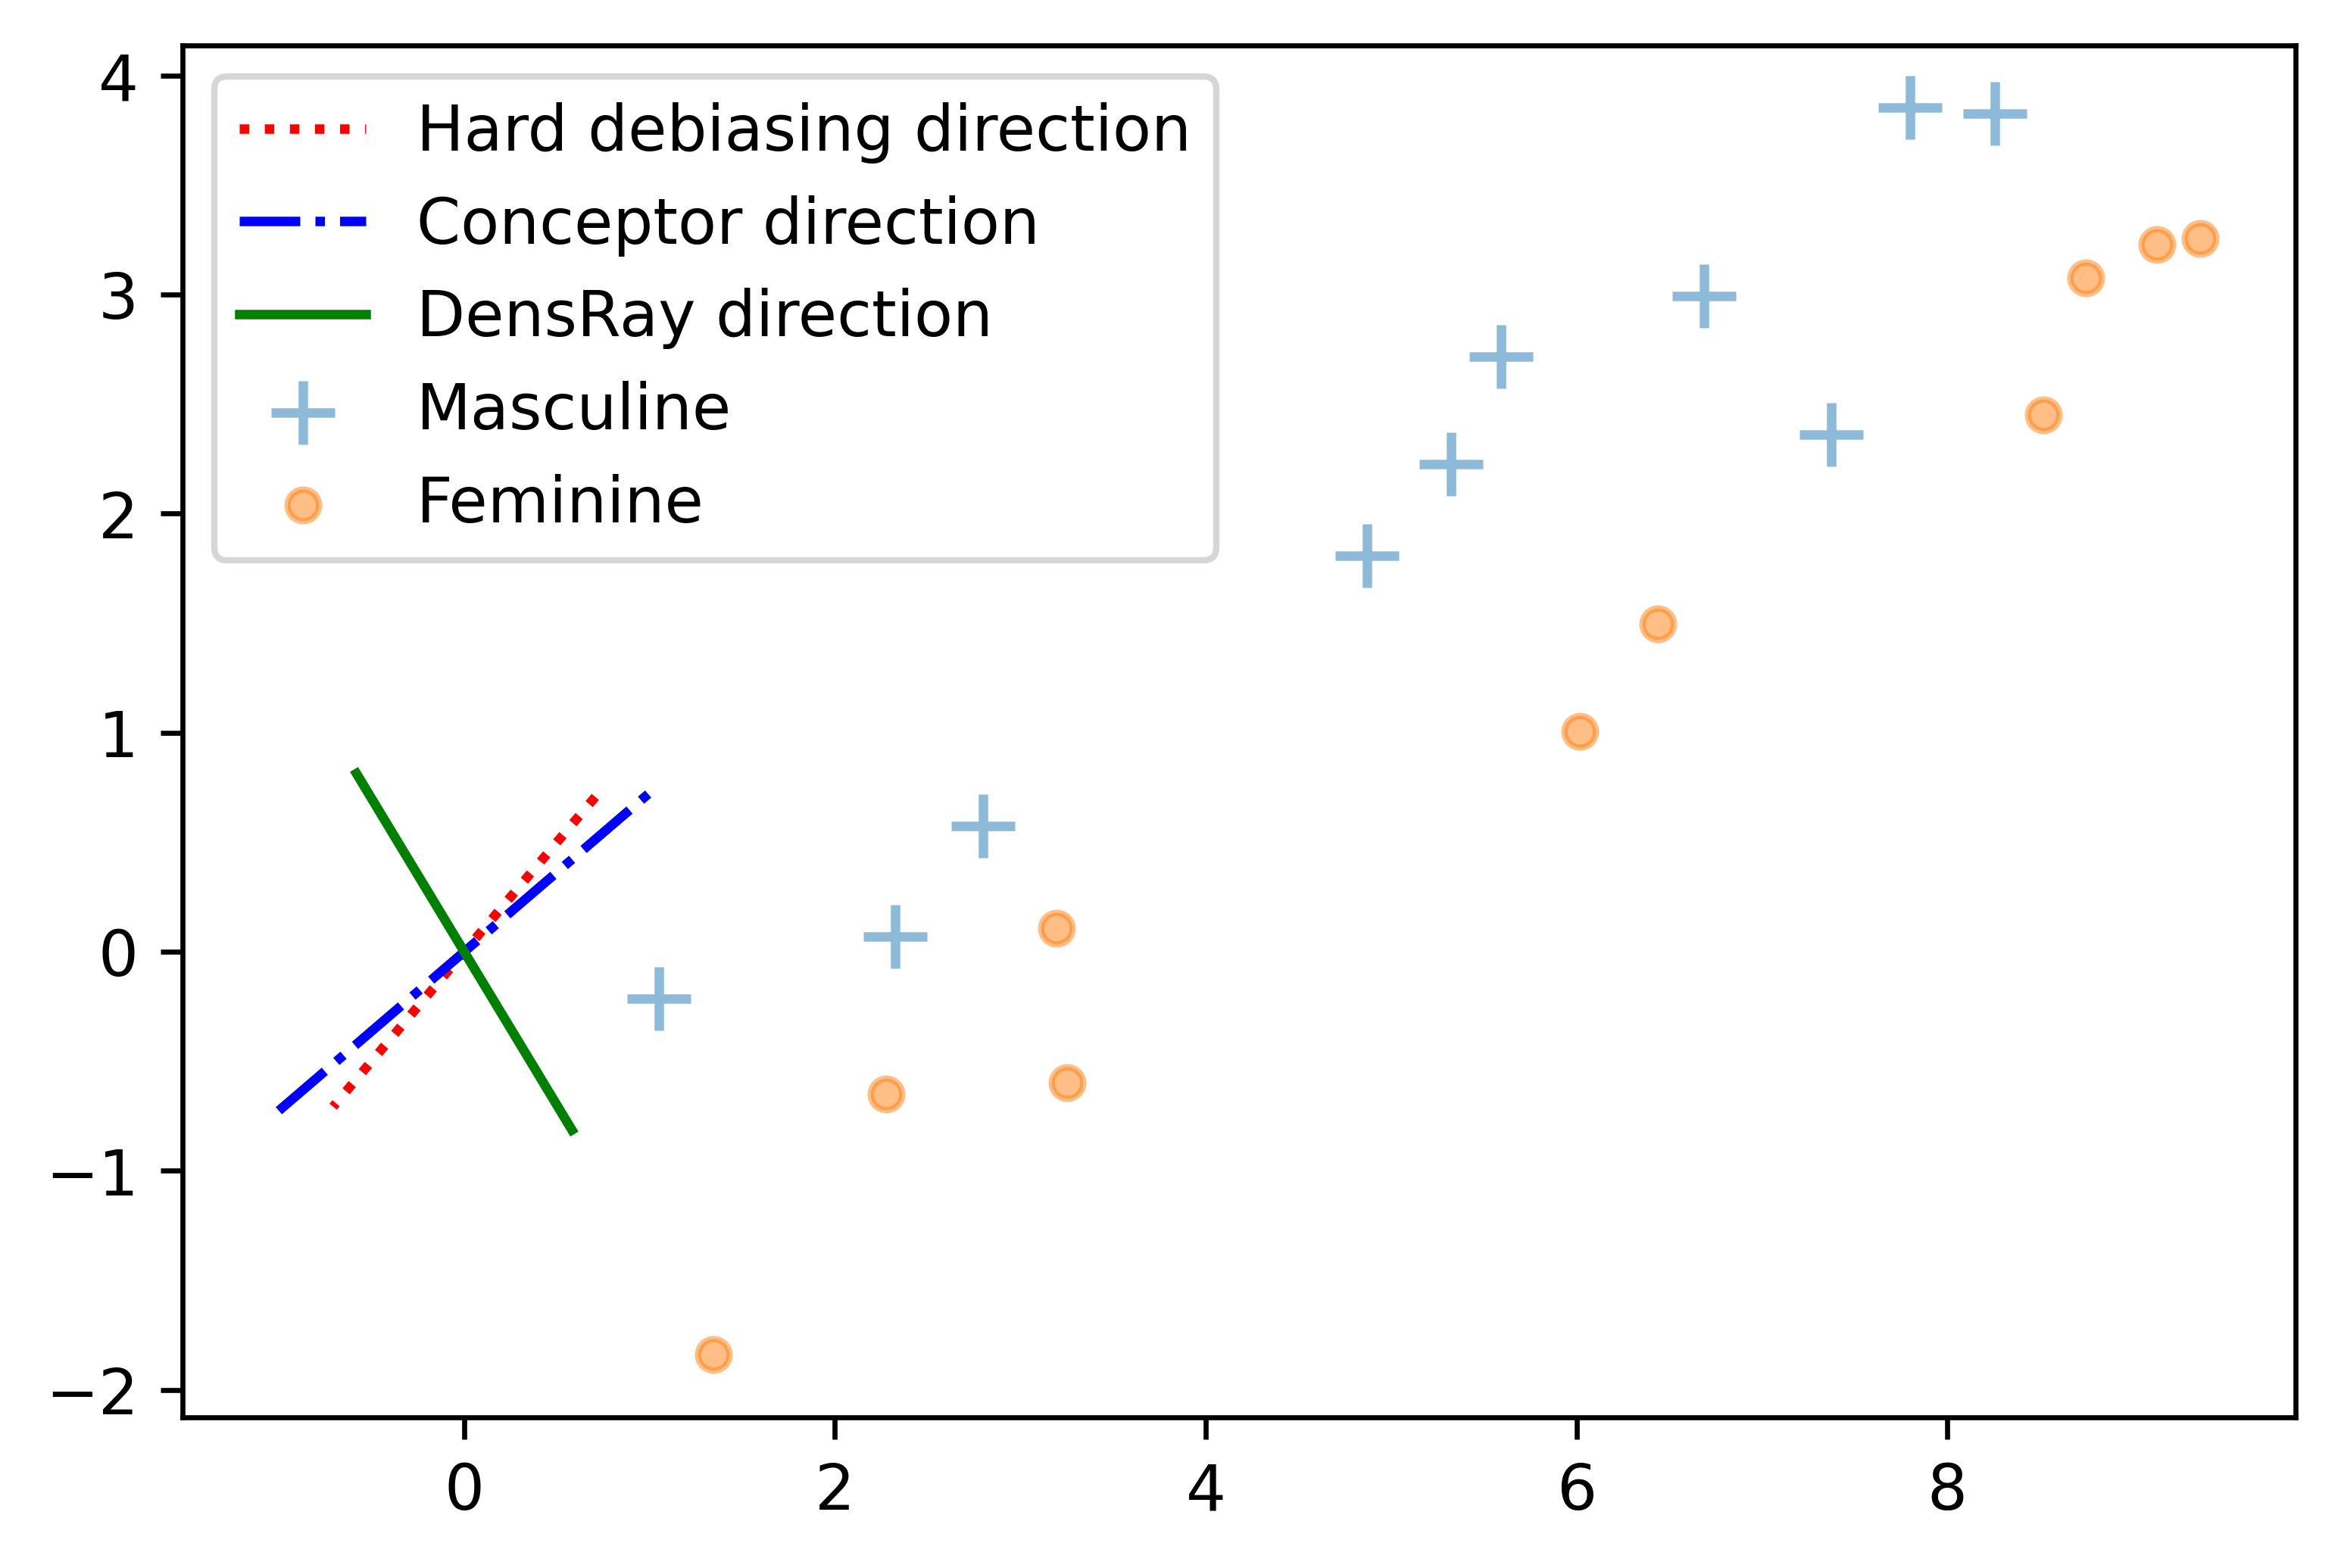
\includegraphics[width=0.5\linewidth]{examples.png}
	\caption{Gender direction on gendered words.}
	\figlabel{fig:example}
\end{figure}

\subsection{Adapting DensRay to Contextualized Language Models}
We now describe how we adapt DensRay to contextualized
language models. Given a set of gendered words
$V$, we extract sentences containing a word in $V$ from a
corpus. We run a contextualized language model
with $M$ layers
on each
sentence
$t_1,\ldots,t_j,\ldots,t_n$ (where $t_j \in V$)
and compute the contextualized representations $e^m, 1\leq m
\leq M$ of $t_j$, one for each layer. 
We compute an orthogonal rotation
matrix $Q_m$ for the $m$th BERT layer using \eqref{eq:densray2}.
For debiasing, we set the gender subspace dimensions to $0$ to eliminate or at least reduce gender information that may cause bias. In this paper, we take the first dimension of the rotated space as the gender subspace.

